\documentclass[11pt,a4paper]{article}

% --- Packages ---
\usepackage[utf8]{inputenc}
\usepackage[margin=0.6in, top=0.65in, bottom=0.65in, headheight=18pt]{geometry}
\usepackage[table]{xcolor}
\usepackage{amsmath,amssymb,amsfonts}
\usepackage{graphicx}
\usepackage{tikz}
\usetikzlibrary{calc,positioning,shapes.geometric,patterns,backgrounds,decorations.pathmorphing}
\usepackage[most]{tcolorbox}
\usepackage{enumitem}
\usepackage{booktabs}
\usepackage{tabularx}
\usepackage{fancyhdr}
\usepackage{titlesec}
\usepackage{fontawesome5}
\usepackage{lastpage}
\usepackage{helvet}
\renewcommand{\familydefault}{\sfdefault}
\usepackage{microtype}
\usepackage[hidelinks]{hyperref}

% --- Color Palette (Modern STEM Theme) ---
\definecolor{NavyMain}{HTML}{1E3A8A}
\definecolor{TealAccent}{HTML}{0D9488}
\definecolor{AmberWarm}{HTML}{D97706}
\definecolor{CharcoalText}{HTML}{1F2937}
\definecolor{LightBg}{HTML}{F8FAFC}
\definecolor{BorderGray}{HTML}{CBD5E1}
\definecolor{SoftTealBg}{HTML}{F0FDFA}
\definecolor{SoftAmberBg}{HTML}{FFFBEB}

% --- Document Setup ---
\color{CharcoalText}
\pagestyle{fancy}
\fancyhf{}
\rhead{\small\color{NavyMain}\textbf{Oakridge Academy} \:\textbar\: AP STEM Series}
\lhead{\small\color{CharcoalText}Problem Set \#4: Waves, Energy \& Thermodynamics}
\rfoot{\small\color{CharcoalText}Page \thepage\ of \pageref{LastPage}}
\lfoot{\small\color{CharcoalText}Student Name: \underline{\hspace{3.8cm}} \quad Period: \underline{\hspace{1.2cm}}}
\renewcommand{\headrulewidth}{0.4pt}
\renewcommand{\footrulewidth}{0.4pt}

% --- Section Header Styling ---
\titleformat{\section}
  {\color{NavyMain}\normalfont\large\bfseries}
  {\thesection}{0.8em}{}
  [\color{TealAccent}\titlerule]

\titleformat{\subsection}
  {\color{TealAccent}\normalfont\normalsize\bfseries}
  {\thesubsection}{0.8em}{}

% --- Custom tcolorbox Styles ---
\tcbset{
  basebox/.style={
    enhanced,
    arc=3pt,
    boxrule=0.8pt,
    fonttitle=\bfseries,
    coltitle=white,
    colback=LightBg,
    colframe=NavyMain
  },
  infobox/.style={
    enhanced,
    arc=3pt,
    boxrule=0.8pt,
    colback=SoftTealBg,
    colframe=TealAccent,
    fonttitle=\bfseries\color{TealAccent},
    top=3pt, bottom=3pt, left=8pt, right=8pt,
    title={\faInfoCircle\:\: Assignment Overview \& Guidelines}
  },
  formulabox/.style={
    enhanced,
    arc=3pt,
    boxrule=0.8pt,
    colback=SoftAmberBg,
    colframe=AmberWarm,
    fonttitle=\bfseries\color{AmberWarm},
    top=3pt, bottom=3pt, left=8pt, right=8pt,
    title={\faLightbulb\:\: Essential Reference Equations \& Constants}
  },
  workspace/.style={
    enhanced,
    arc=3pt,
    boxrule=0.6pt,
    colback=white,
    colframe=BorderGray,
    coltitle=NavyMain,
    fonttitle=\scriptsize\bfseries,
    top=2pt, bottom=2pt, left=6pt, right=6pt,
    title={\faPen\:\: Solution Workspace (Show all steps, formulas, and units)}
  }
}

\begin{document}

% ==========================================
% PAGE 1: HEADER, INSTRUCTIONS & MULTIPLE CHOICE
% ==========================================
\begin{tcolorbox}[
  enhanced,
  colback=NavyMain,
  colframe=NavyMain,
  arc=4pt,
  boxrule=0pt,
  top=3pt, bottom=3pt, left=8pt, right=8pt
]
  \begin{minipage}[c]{0.68\textwidth}
    \color{white}
    {\large \textbf{OAKRIDGE ACADEMY OF SCIENCE \& TECHNOLOGY}} \\[1pt]
    {\small \textbf{Department of Physics \& Chemical Sciences}} \\[2pt]
    {\Large \textbf{Problem Set \#4: Integrated STEM}} \\[1pt]
    {\footnotesize Course: AP Physics \& Chemistry \quad\textbar\quad Instructor: Dr. E. Vance}
  \end{minipage}%
  \hfill
  \begin{minipage}[c]{0.28\textwidth}
    \begin{tcolorbox}[
      colback=white,
      colframe=TealAccent,
      arc=3pt,
      boxrule=1pt,
      halign=center,
      top=2pt, bottom=2pt
    ]
      \color{NavyMain}
      \textbf{TOTAL POINTS: 100} \\[1pt]
      \small Score: \underline{\hspace{1.0cm}} / 100 \\[1pt]
      \scriptsize \faCalendar\:\: Due: Oct 28, 2026
    \end{tcolorbox}
  \end{minipage}
\end{tcolorbox}

\vspace{0.08cm}

\begin{tcolorbox}[infobox]
  \begin{minipage}[t]{0.48\textwidth}
    \begin{itemize}[leftmargin=1.1em, label=\textcolor{TealAccent}{\scriptsize\faCheckCircle}, itemsep=0pt]
      \item \textbf{Calculators:} Scientific/graphing allowed (TI-84 style).
      \item \textbf{Show Work:} Full credit requires setup, values, and units.
    \end{itemize}
  \end{minipage}%
  \hfill
  \begin{minipage}[t]{0.48\textwidth}
    \begin{itemize}[leftmargin=1.1em, label=\textcolor{TealAccent}{\scriptsize\faCheckCircle}, itemsep=0pt]
      \item \textbf{Integrity:} Concepts may be discussed; work must be unique.
      \item \textbf{Submission:} Place in Bin B by 3:15 PM on due date.
    \end{itemize}
  \end{minipage}
\end{tcolorbox}

\vspace{0.08cm}

\section{Section I: Multiple Choice \& Conceptual Analysis (20 Points)}
\textit{Select the best response for each item. Encircle your choice and write a brief 1-sentence justification.}

\vspace{0.08cm}

\begin{enumerate}[label=\textbf{Q\arabic*.}, leftmargin=1.5em, itemsep=0.15em]

  \item A monochrome beam of green laser light ($\lambda = 532\text{ nm}$) transitions from air ($n = 1.00$) into crown glass ($n = 1.52$). Which statement correctly describes the change in the wave's properties?
  \begin{enumerate}[label=(\Alph*), leftmargin=1.8em, itemsep=0pt]
    \item The frequency decreases, while the wavelength remains constant.
    \item The frequency remains constant, while the wavelength decreases to approximately $350\text{ nm}$.
    \item The speed increases to $4.56 \times 10^8\text{ m/s}$, and frequency increases.
    \item Both speed and frequency decrease by a factor of $1.52$.
  \end{enumerate}
  \textit{Justification:} \underline{\hspace{12.5cm}}

  \item A $2.50\text{ kg}$ aluminum block ($90.0^\circ\text{C}$) is placed into $1.00\text{ kg}$ of water ($20.0^\circ\text{C}$) in an insulated calorimeter. What is the equilibrium temperature $T_f$? ($c_{\text{Al}} = 900\text{ J/(kg}\cdot^\circ\text{C)}$, $c_{\text{w}} = 4184\text{ J/(kg}\cdot^\circ\text{C)}$).
  \begin{enumerate}[label=(\Alph*), leftmargin=1.8em, itemsep=0pt]
    \item $35.0^\circ\text{C}$ \quad (B) $44.5^\circ\text{C}$ \quad (C) $55.0^\circ\text{C}$ \quad (D) $68.2^\circ\text{C}$
  \end{enumerate}
  \textit{Justification:} \underline{\hspace{12.5cm}}

  \item Refer to the energy level schematic for synthetic atom \textbf{Vertex-9}. A photon of frequency $f = 6.18 \times 10^{14}\text{ Hz}$ is emitted during electronic relaxation.

  \begin{center}
  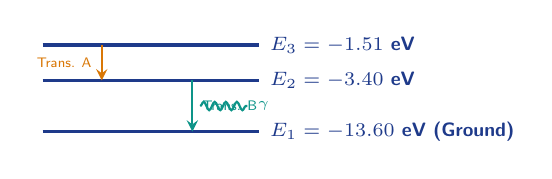
\begin{tikzpicture}[scale=0.50]
    \draw[very thick, NavyMain] (0,2.2) -- (5.5,2.2) node[right, NavyMain] {\scriptsize\textbf{$E_3 = -1.51\text{ eV}$}};
    \draw[very thick, NavyMain] (0,1.3) -- (5.5,1.3) node[right, NavyMain] {\scriptsize\textbf{$E_2 = -3.40\text{ eV}$}};
    \draw[very thick, NavyMain] (0,0) -- (5.5,0) node[right, NavyMain] {\scriptsize\textbf{$E_1 = -13.60\text{ eV}$ (Ground)}};
    \draw[->, >=stealth, thick, AmberWarm] (1.5,2.2) -- (1.5,1.3) node[midway, left, AmberWarm] {\tiny Trans. A};
    \draw[->, >=stealth, thick, TealAccent] (3.8,1.3) -- (3.8,0) node[midway, right, TealAccent] {\tiny Trans. B};
    \draw[thick, TealAccent, decoration={snake, amplitude=1.5pt, segment length=4pt}, decorate] (4.0, 0.65) -- (5.2, 0.65) node[right] {\tiny $\gamma$};
  \end{tikzpicture}
  \end{center}

  Which quantum transition generated this emitted photon?
  \begin{enumerate}[label=(\Alph*), leftmargin=1.8em, itemsep=0pt]
    \item $E_3 \rightarrow E_2$ \quad (B) $E_2 \rightarrow E_1$ \quad (C) $E_3 \rightarrow E_1$ \quad (D) $E_1 \rightarrow \infty$
  \end{enumerate}
  \textit{Justification:} \underline{\hspace{12.5cm}}

  \item The synthesis of ammonia ($N_2 + 3H_2 \rightleftharpoons 2NH_3$) has $E_a = 145\text{ kJ/mol}$. When a catalyst (\textbf{Nexa Corp}) is added:
  \begin{enumerate}[label=(\Alph*), leftmargin=1.8em, itemsep=0pt]
    \item $\Delta H^\circ$ becomes more negative.
    \item Both forward and reverse $E_a$ are lowered by equal energy amounts.
    \item The equilibrium yield of $NH_3$ increases at constant temperature.
    \item Forward $E_a$ decreases while reverse $E_a$ increases.
  \end{enumerate}
  \textit{Justification:} \underline{\hspace{12.5cm}}

\end{enumerate}

\newpage

% ==========================================
% PAGE 2: PROBLEM 5 (OPTICS)
% ==========================================
\section{Section II: Structured Quantitative Problems (45 Points)}

\begin{tcolorbox}[formulabox]
  \scriptsize
  \begin{tabularx}{\textwidth}{X X X}
    \textbf{Wave Mechanics:} & \textbf{Thermodynamics:} & \textbf{Constants:} \\
    $v = f \lambda \quad\mid\quad d \sin\theta = m \lambda$ & $Q = m c \Delta T \quad\mid\quad Q = n \Delta H$ & $c = 3.00 \times 10^8\text{ m/s}$ \\
    $n_1 \sin\theta_1 = n_2 \sin\theta_2$ & $\Delta G^\circ = \Delta H^\circ - T\Delta S^\circ$ & $h = 6.626 \times 10^{-34}\text{ J}\cdot\text{s} \quad\mid\quad R = 8.314\text{ J/(mol}\cdot\text{K)}$
  \end{tabularx}
\end{tcolorbox}

\vspace{0.08cm}

\subsection*{Problem 5: Optics \& Wave Interference Analysis (20 Points)}

A double-slit experiment is set up with a red laser ($\lambda = 632.8\text{ nm}$). The slit separation is $d = 0.180\text{ mm}$ and the distance to the screen is $L = 2.40\text{ m}$.

\begin{center}
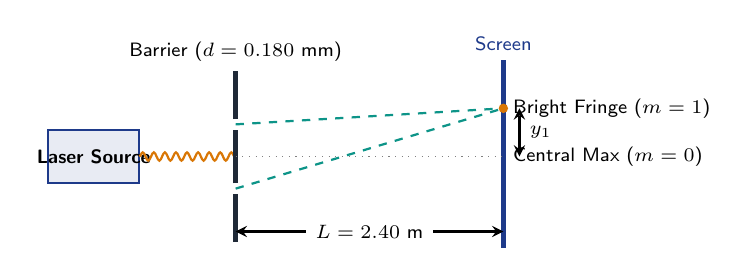
\begin{tikzpicture}[scale=0.68]
  % Laser source
  \draw[fill=NavyMain!10, draw=NavyMain, thick] (-0.5, 0.6) rectangle (1.2, 1.6);
  \node at (0.35, 1.1) {\scriptsize\textbf{Laser Source}};
  
  % Beam
  \draw[thick, AmberWarm, decoration={snake, amplitude=1.5pt, segment length=4pt}, decorate] (1.2, 1.1) -- (3.0, 1.1);
  
  % Double slit barrier
  \draw[ultra thick, CharcoalText] (3.0, -0.5) -- (3.0, 0.4);
  \draw[ultra thick, CharcoalText] (3.0, 0.6) -- (3.0, 1.6);
  \draw[ultra thick, CharcoalText] (3.0, 1.8) -- (3.0, 2.7);
  \node[above] at (3.0, 2.7) {\scriptsize Barrier ($d = 0.180\text{ mm}$)};
  
  % Screen
  \draw[ultra thick, NavyMain] (8.0, -0.6) -- (8.0, 2.9);
  \node[above, NavyMain] at (8.0, 2.9) {\scriptsize Screen};
  
  % Rays to m=1 fringe
  \draw[dashed, TealAccent, thick] (3.0, 0.5) -- (8.0, 2.0);
  \draw[dashed, TealAccent, thick] (3.0, 1.7) -- (8.0, 2.0);
  \draw[fill=AmberWarm, draw=none] (8.0, 2.0) circle (2.5pt) node[right, black] {\scriptsize Bright Fringe ($m=1$)};
  
  % Center line
  \draw[dotted, gray] (3.0, 1.1) -- (8.0, 1.1) node[right, black] {\scriptsize Central Max ($m=0$)};
  
  % Dimension L
  \draw[<->, >=stealth, thick] (3.0, -0.3) -- (8.0, -0.3) node[midway, fill=white] {\scriptsize $L = 2.40\text{ m}$};
  % Dimension y
  \draw[<->, >=stealth, thick] (8.3, 1.1) -- (8.3, 2.0) node[midway, right] {\scriptsize $y_1$};
\end{tikzpicture}
\end{center}

\begin{enumerate}[label=\alph*), leftmargin=1.5em, itemsep=0.15em]
  \item Calculate the angular displacement $\theta_1$ (in degrees) for the first-order bright fringe ($m = 1$).
  \item Determine the distance $y_1$ on the screen from the central maximum to the first bright fringe.
  \item If submerged in water ($n = 1.333$), calculate the new fringe spacing $y_1'$ and explain the physical cause.
\end{enumerate}

\begin{tcolorbox}[workspace, height=12.0cm]
  % Workspace Problem 5
\end{tcolorbox}

\newpage

% ==========================================
% PAGE 3: PROBLEM 6 (CALORIMETRY)
% ==========================================
\subsection*{Problem 6: Calorimetry \& Chemical Enthalpy (25 Points)}

A chemist at \textbf{Synapse Materials Research} conducts a bomb calorimetry experiment to determine the molar heat of combustion of liquid ethanol ($\text{C}_2\text{H}_5\text{OH}$). A $1.84\text{ g}$ sample is ignited in a calorimeter containing $1200\text{ g}$ of water.

Reaction equation:
\[
\text{C}_2\text{H}_5\text{OH}(l) + 3\text{O}_2(g) \longrightarrow 2\text{CO}_2(g) + 3\text{H}_2\text{O}(l)
\]
The system temperature rises from $22.40^\circ\text{C}$ to $33.15^\circ\text{C}$. The bomb calorimeter heat capacity is $C_{\text{calorimeter}} = 850\text{ J/}^\circ\text{C}$.

\vspace{0.08cm}

\begin{tcolorbox}[basebox, colframe=TealAccent, title={\faDatabase\:\: Experimental Dataset Summary}]
  \centering
  \scriptsize
  \begin{tabularx}{0.95\textwidth}{X c c}
    \toprule
    \textbf{Parameter} & \textbf{Symbol / Variable} & \textbf{Recorded Value} \\
    \midrule
    Mass of Ethanol Sample & $m_{\text{ethanol}}$ & $1.84\text{ g}$ \\
    Molar Mass of Ethanol & $M_{\text{ethanol}}$ & $46.07\text{ g/mol}$ \\
    Mass of Water Bath & $m_{\text{water}}$ & $1200\text{ g}$ \\
    Specific Heat of Water & $c_{\text{water}}$ & $4.184\text{ J/(g}\cdot^\circ\text{C)}$ \\
    Calorimeter Heat Capacity & $C_{\text{calorimeter}}$ & $850\text{ J/}^\circ\text{C}$ \\
    Initial Temperature & $T_i$ & $22.40^\circ\text{C}$ \\
    Final Temperature & $T_f$ & $33.15^\circ\text{C}$ \\
    \bottomrule
  \end{tabularx}
\end{tcolorbox}

\vspace{0.08cm}

\begin{enumerate}[label=\alph*), leftmargin=1.5em, itemsep=0.15em]
  \item Calculate the total thermal energy $Q_{\text{total}}$ absorbed by the water bath and calorimeter vessel.
  \item Calculate the number of moles of ethanol consumed in this reaction trial.
  \item Determine the experimental molar enthalpy of combustion ($\Delta H_{\text{comb}}$) in $\text{kJ/mol}$ with proper sign.
  \item Given accepted $\Delta H_{\text{comb}}^\circ = -1367\text{ kJ/mol}$, calculate the experimental percent error.
\end{enumerate}

\begin{tcolorbox}[workspace, height=12.0cm]
  % Workspace Problem 6
\end{tcolorbox}

\newpage

% ==========================================
% PAGE 4: ADVANCED FREE RESPONSE CHALLENGE
% ==========================================
\section{Section III: Advanced Free-Response Design Challenge (35 Points)}

\begin{tcolorbox}[basebox, colframe=NavyMain, title={\faAtom\:\: Scenario: Photovoltaic-Thermal Hybrid Cell for Space Probes}]
  Engineers at \textbf{Nimbus Clean Energy Labs} are evaluating a radioisotope thermal generator (RTG) coupled with a thermoelectric Seebeck array to produce electricity from the decay heat of Plutonium-238 ($^{238}\text{Pu}$).
\end{tcolorbox}

\vspace{0.05cm}

\begin{center}
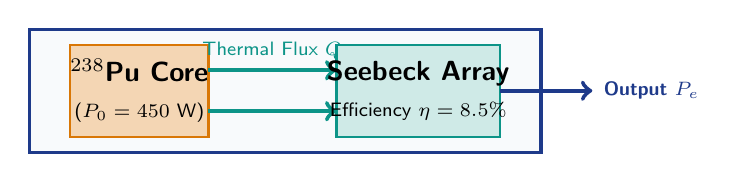
\begin{tikzpicture}[scale=0.65]
  % Container box
  \draw[very thick, NavyMain, fill=LightBg] (0,0) rectangle (10,2.4);
  
  % Core RTG
  \draw[thick, fill=AmberWarm!30, draw=AmberWarm] (0.8,0.3) rectangle (3.5,2.1);
  \node[align=center] at (2.15,1.2) {\textbf{$^{238}\text{Pu}$ Core}\\[1pt]\scriptsize ($P_0 = 450\text{ W}$)};
  
  % Thermal Pipes
  \draw[ultra thick, TealAccent, ->] (3.5, 1.6) -- (6.0, 1.6) node[midway, above] {\scriptsize Thermal Flux $Q$};
  \draw[ultra thick, TealAccent, ->] (3.5, 0.8) -- (6.0, 0.8);
  
  % Thermoelectric Generator
  \draw[thick, fill=TealAccent!20, draw=TealAccent] (6.0, 0.3) rectangle (9.2, 2.1);
  \node[align=center] at (7.6, 1.2) {\textbf{Seebeck Array}\\[1pt]\scriptsize Efficiency $\eta = 8.5\%$};
  
  % Electrical output
  \draw[ultra thick, NavyMain, ->] (9.2, 1.2) -- (11.0, 1.2) node[right] {\scriptsize\textbf{Output $P_e$}};
\end{tikzpicture}
\end{center}

\vspace{0.02cm}

\subsection*{Part A: Radioactive Decay Kinematics (12 Points)}
Plutonium-238 decays via alpha particle emission ($\alpha$) with half-life $T_{1/2} = 87.7\text{ years}$: \, $^{238}_{94}\text{Pu} \longrightarrow \, ^{A}_{Z}\text{X} \,+\, ^{4}_{2}\text{He}$.

\begin{enumerate}[label=\arabic*., leftmargin=1.5em, itemsep=0.08em]
  \item Identify daughter nuclide $^{A}_{Z}\text{X}$ (atomic number $Z$, mass number $A$, chemical symbol).
  \item Calculate the decay constant $\lambda$ of Plutonium-238 in $\text{s}^{-1}$.
  \item Calculate remaining thermal power output after $25.0\text{ years}$ ($P_0 = 450\text{ W}$).
\end{enumerate}

\begin{tcolorbox}[workspace, height=2.8cm]
\end{tcolorbox}

\subsection*{Part B: System Efficiency \& Power Conversion (13 Points)}

\begin{enumerate}[label=\arabic*., leftmargin=1.5em, itemsep=0.08em]
  \item Given $\eta = 8.50\%$, calculate initial electrical power output $P_e$ (Watts) at $t = 0$.
  \item Telemetry requires minimum continuous power $28.0\text{ W}$. Calculate lifespan in years before dropping below threshold.
\end{enumerate}

\begin{tcolorbox}[workspace, height=2.8cm]
\end{tcolorbox}

\subsection*{Part C: Conceptual Synthesis \& Design Evaluation (10 Points)}
Explain two physical mechanisms causing RTG system power output to degrade faster than radioisotope decay kinetics predict.

\begin{tcolorbox}[workspace, height=2.0cm]
\end{tcolorbox}

\vspace{0.05cm}

\begin{center}
  \color{TealAccent}
  \rule{0.5\textwidth}{0.5pt} \\[1pt]
  \scriptsize\textbf{--- END OF PROBLEM SET \#4 ---}
\end{center}

\end{document}
